\documentclass[a4papper, 11pt]{article}

\title{-- Digital Microelectronics --- SoundLoc -- \\ Localication of Soundsources by cross-correlating three $\Sigma\Delta$-microphon signals}
\author{Stefan Kull, Roy Seitz, Marco Zollinger}

\usepackage[T1]{fontenc}			%umlaute als eigene Zeichen
\usepackage[latin1]{inputenc}	%umlaute erkennen
\usepackage{lmodern}
\usepackage{amsmath} 					%mathematischen Textsatz.
\usepackage{amssymb}					%	-Erweiterte math. Sonderzeichen
\usepackage{dsfont}						%	-Mengen			
\usepackage[english]{babel}
\usepackage{textgreek}
\usepackage{siunitx}
\usepackage{graphicx}
\usepackage{caption}			%f�r \captionof

\usepackage[
	pdftitle={SoundLoc -- Digital Microelectronics Project},						%Titel des PDF Dokuments.
	pdfauthor={Stefan Kull, Roy Seitz, Marco Zollinger},									%Autor des PDF Dokuments.
	pdfsubject={Sound localication useing cross correlation of three microphones},		%Thema des PDF Dokuments.
	pdfcreator={LaTeX with hyperref and KOMA-Script},		%Erzeuger des PDF Dokuments.
	pdfkeywords={Cross correlatin, CIC, IP, AXI4\_Lite interface},						%auch f�r PDF Dokumente indexiert
	%	pdfpagemode=UseOutlines,								%Inhaltsverzeichnis anzeigen beim ffnen
	pdfdisplaydoctitle=true,								%Dokumenttitel statt Dateiname anzeigen.
	pdflang=en,												%Sprache des Dokuments.
	plainpages=false,
	hidelinks,												%keine Box um Links
	%	bookmarksopen.											%toc beim �ffnen expandiert
	pdfpagelabels
]{hyperref}

\usepackage[
%includeheadfoot,		%Kopf- und Fusszeilen verwenden
%headheight=15pt,		%H�he der Kopfzeile
left=30mm,				%abstand von Seitenraendern
right=30mm,				%
top=20mm,
bottom=20mm,
%			twoside
]{geometry}


\usepackage{subcaption}

\begin{document}
\maketitle
\setcounter{tocdepth}{2}

\begin{figure}[htbp]
	\begin{subfigure}{0.5\textwidth}
		\centering
		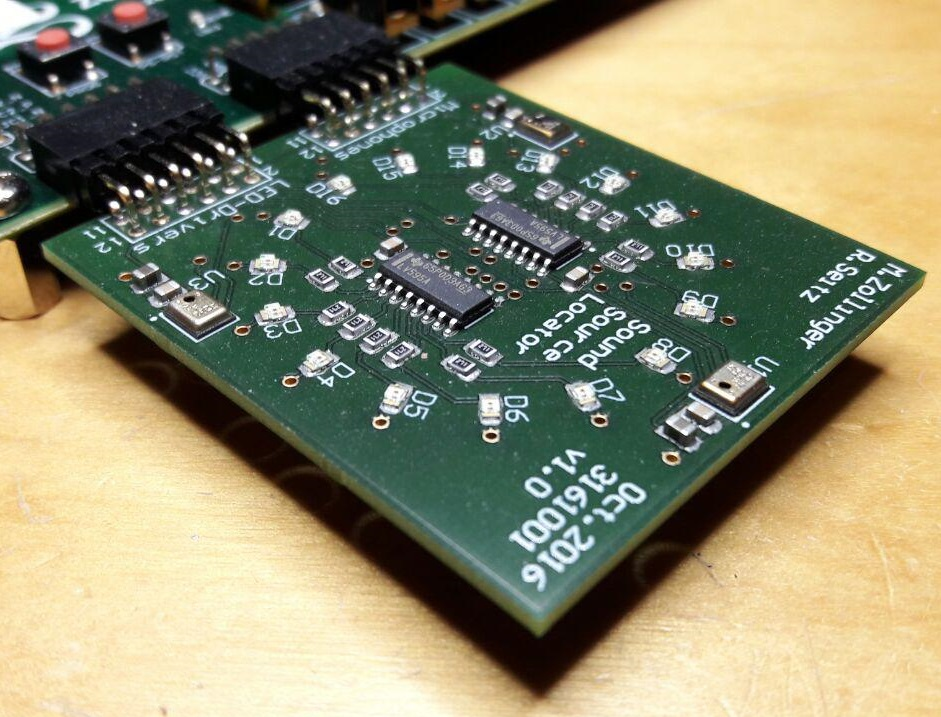
\includegraphics[scale=.4]{./block_diagram/pcb.jpg}
		\captionof{figure}{Top Level Block Diagram}
		\label{fig::top_block}
	\end{subfigure}
	\begin{subfigure}{0.5\textwidth}
		\centering
		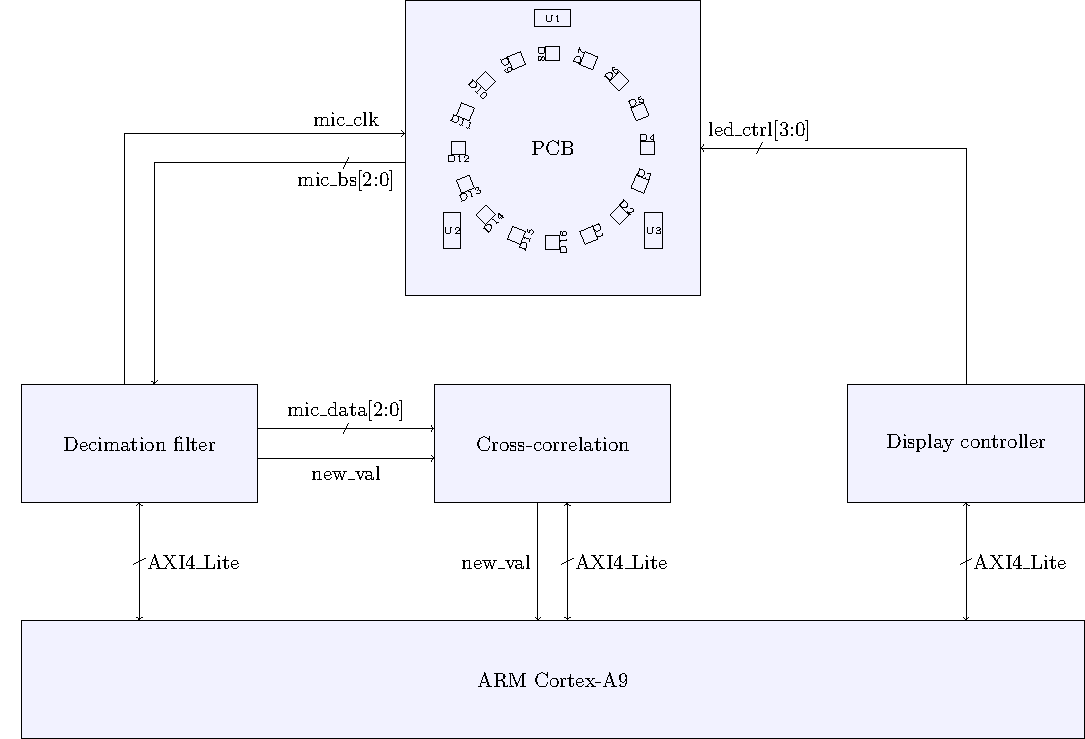
\includegraphics[scale=.4]{./block_diagram/system_top.pdf}
		\captionof{figure}{Top Level Block Diagram}
		\label{fig::top_block}
	\end{subfigure}
	\caption{Caption for this figure with two images}
	\label{fig:image2}
\end{figure}

 
\section{Overview}
Sound travels at a speed of approximately $c\approx \SI{340}{\meter\per\s}$.
Using multiple microphones at well known locations allows calculating the direction from which the sound came.
Three microphones are placed in an equilateral triangle of 42 mm of side length.
A circle of 16 LEDs is placed on the same PCB to indicate the direction.
Because only the direction in two dimensions is of interest, three microphones are sufficient.
The microphone operate at approximately \SI{3.2}{\mega\hertz} using $\Sigma\Delta$-modulation.
They output their bitstream directly without any digital filtering or decimation.
Figure \ref{fig::top_block} shows a block diagram of the whole system.

The bitstream is filtered by a IP block, configurable by software via AXI4 Lite interface.
This block contains a CIC filter of configurable order and decimation rate with a differential Delay of $M=1$.
An additional IIR filter can be enabled to remove the DC component of the signals.
See Section \ref{sec::filter} for further information.

From the decimated data, the cross correlation is calculated to find the signal delay between the microphones due to finite sound speed.
This is done by another IP block, also configurable over AXI4 Lite.
See section \ref{sec::xcorr} for further information.

These delays are read by the CPU, which calculates the direction of the sound source. 
It basically consists of a base transform from microphone to Cartesian coordinates and calculating the inverse tangent of these coordinates.
This is described in section \ref{sec::software}.

The Angle is mapped to one of the 16 LED and then fed to another IP block that displays the direction.
It consists of a simple 16 bit shift register that illuminates the corresponding LED.
For this, see section \ref{sec::display}.



\section{Decimation Filter}
\label{sec::filter}


\section{Cross Correlation}
\label{sec::xcorr}


\section{Software}
\label{sec::software}

\section{LED Display}
\label{sec::display}

The 16 LEDs are controlled by two 8-bit shift registers.
The LED nearest to the calculated direction is switched on every cycle.
Due to remaining noise and fast processing speed, interpolation seemingly happens by illuminating neighboring LEDs alternatively.

\end{document}